\documentclass[journal]{IEEEtran}
\usepackage{amsmath,amssymb}
\usepackage{cite}
\usepackage{graphicx}
\usepackage{array}
\newcolumntype{P}[1]{>{\raggedright\arraybackslash}p{#1}}
\usepackage{tikz}
\usetikzlibrary{positioning,arrows.meta}
\usepackage[hidelinks]{hyperref}

\begin{document}

\title{User Mobility in Edge Caching: A Survey of Models, Their Effect on Caching Gain, and a Unified Benchmark}

\author{Sameh~Hosny and John~Tadrous%
\thanks{S. Hosny is with the Electrical and Computer Engineering Department, American University of Armenia, Yerevan, Armenia (e-mail: sameh.hosny@aua.am).}%
\thanks{J. Tadrous is with the Department of Electrical and Computer Engineering, Gonzaga University, Spokane, WA 99258, USA (e-mail: tadrous@gonzaga.edu).}}

\maketitle

\begin{abstract}
Edge caching stores popular content at small base stations, user devices, roadside units and unmanned aerial vehicles, close to the users who request it. Users move, and the literature models their movement in many ways, from Poisson snapshots and random waypoint to Markov chains, contact processes and recorded traces. The reported effect of mobility on the caching gain varies just as widely: some studies find that mobility raises the gain, others that it lowers it. This survey reviews how user mobility is represented in edge caching and how it changes the gain. We group mobility models into five families, classify 24 caching studies across cellular, device-to-device (D2D), vehicular and UAV networks by how their caching decisions use mobility, and explain the conflicting findings through four mechanisms: new contacts and caches, interrupted delivery, duplication versus diversity, and unpredictable movement. Only 9 of the 24 studies vary mobility in their evaluation. We then present an open MATLAB benchmark that fixes the network, content and caching policies and changes only the mobility model. Across six moving models at the same nominal speed, the gain of one mobility-aware placement over most-popular caching ranges from 0.7\% to 24.3\%, and changing only the D2D transfer time turns the effect of mobility from positive to non-monotone to negative. Measured mobility statistics explain this spread better than the model name or the speed: the small-cell gain grows with the number of cells a user can reach before the deadline, and a closed-form prediction that uses only the contact-length distribution reproduces the D2D offloading ratio of all 210 tested configurations with a mean error of 0.004. A snapshot hit ratio and a delivery-aware hit ratio rank the placements in opposite orders, and when most users are static, a placement trained on moving users falls below most-popular caching. We close with reporting recommendations and open problems.
\end{abstract}

\begin{IEEEkeywords}
Edge caching, user mobility, mobility models, D2D caching, vehicular networks, UAV caching, proactive caching, benchmark.
\end{IEEEkeywords}

% ============================================================
% Section 1: Introduction
% ============================================================

\section{Introduction}
\label{sec:intro}

Caching popular content close to users is a standard way to cut backhaul traffic and delivery delay in wireless networks. Small base stations, user devices, roadside units and UAVs can all hold content, and a decade of work has shown how to decide what each cache should store~\cite{shanmugam2013femtocaching,golrezaei2013femtocaching,maddahali2014fundamental,bastug2014living,paschos2018role}. Much of that work assumes that each user stays attached to the same caches while it is served.

A moving user changes the problem in two ways. Over the placement time scale it visits several caches, so it can reach the union of their content. Over the delivery time scale it may leave a cell, or lose contact with a peer, before the file arrives. Papers that account for mobility model it as a random displacement~\cite{krishnan2017mobility}, a Markov chain over cells~\cite{poularakis2013exploiting,ozfatura2020mobility}, contact processes between devices~\cite{wang2017mobility,wang2018exploiting}, a street grid~\cite{alnagar2019city} or recorded traces~\cite{chen2017sky,choi2023deep}, and they disagree on whether mobility raises the gain~\cite{wang2018exploiting} or lowers it~\cite{jarray2016mobility}.

Mobile ad hoc networking faced the same situation twenty years ago, when Camp \emph{et al.}~\cite{camp2002survey} showed that the choice of mobility model alone changed the reported routing performance. Edge caching has not had this comparison. Of the 24 caching studies we coded, only 7 vary a mobility parameter in their evaluation, and none tests a placement under a mobility model other than its own.

\subsection{Related Surveys}
\label{subsec:related}

Table~\ref{tab:surveys} lists the closest surveys. Overviews of wireless caching~\cite{bastug2014living,paschos2018role} treat mobility as one consideration among many; the others review mobility-aware caching~\cite{wang2016framework}, mobility prediction~\cite{bui2017survey} or D2D mobility models~\cite{waqas2020survey}. None compares mobility models against the caching gain under common conditions.

\begin{table*}[t]
\centering
\caption{Related surveys and tutorials, as assessed by the authors (--: not a focus)}
\label{tab:surveys}
\footnotesize
\renewcommand{\arraystretch}{1.15}
\begin{tabular}{llllll}
\hline
Work & Year & Scope & Mobility models reviewed & Effect on caching gain & Common comparison \\
\hline
\cite{camp2002survey} & 2002 & Mobility models for ad hoc networks & Synthetic & No (routing only) & Routing, several models \\
\cite{bastug2014living} & 2014 & Proactive caching in 5G & -- & -- & No \\
\cite{wang2016framework} & 2016 & Mobility-aware caching framework & Spatio-temporal properties & Partly & No \\
\cite{bui2017survey} & 2017 & Anticipatory mobile networking & Prediction methods & Partly & No \\
\cite{paschos2018role} & 2018 & Role of caching in future networks & -- & -- & No \\
\cite{waqas2020survey} & 2020 & Mobility-aware D2D communications & D2D models and traces & No & No \\
This survey & 2026 & User mobility in edge caching & Five families & Four mechanisms & Seven-model benchmark \\
\hline
\end{tabular}
\end{table*}

\subsection{Contributions and Organization}
\label{subsec:contrib}

We ask how user mobility is represented in edge caching (RQ1), where it enters the caching problem (RQ2), how it changes the caching gain (RQ3), whether results are comparable across papers (RQ4) and what is missing (RQ5). After background in Section~\ref{sec:background}, the contributions are:
\begin{enumerate}
\item a taxonomy of mobility models in five families (Section~\ref{sec:models});
\item a classification of 24 caching studies across cellular, D2D, vehicular and UAV networks by model, use of mobility, metric and whether mobility is varied (Section~\ref{sec:problems});
\item four mechanisms that explain the conflicting findings (Section~\ref{sec:effect});
\item an open MATLAB benchmark that changes only the mobility model across seven models and six speeds, and shows which measured mobility statistics determine the gain (Section~\ref{sec:benchmark});
\item reporting recommendations and open problems (Sections~\ref{sec:lessons} and~\ref{sec:open}).
\end{enumerate}
Section~\ref{sec:conclusion} concludes.

\emph{Survey method.} We searched IEEE Xplore, the ACM Digital Library, ScienceDirect, arXiv and Google Scholar for 2013 to 2026, combining caching terms (edge, D2D, proactive, vehicular, UAV caching) with mobility terms (mobility, random waypoint, Markov, trace, sojourn, contact time). Papers were screened by title and abstract and coded for the fields of Table~\ref{tab:corpus}, from the full text where available and otherwise from the abstract; unsupported fields are marked as not coded. Every reference was checked against the publisher, DBLP, an institutional repository or arXiv. % TODO: update counts for the final corpus

% ============================================================
% Section 2: Background
% ============================================================

\section{Background on Edge Caching}
\label{sec:background}

This section fixes the terms used in the rest of the survey: where caches sit, how content is placed and delivered, how popularity is modeled, and which metrics measure the caching gain.

\subsection{Where Caches Sit}
\label{subsec:where}

Caches can sit at four edge tiers, and each sees user mobility differently. Caching deeper in the core is outside our scope.

\emph{Small base stations and helpers.} FemtoCaching~\cite{shanmugam2013femtocaching} places storage at small-cell helpers with weak backhaul and decides which files each helper stores so that users in overlapping coverage areas are served locally. A user who moves between small cells sees the union of several caches over time, which is the starting point of most mobility-aware placement schemes~\cite{poularakis2013exploiting,poularakis2017code,ozfatura2020mobility}.

\emph{User devices.} Devices can cache content and serve each other over D2D links~\cite{golrezaei2013femtocaching}. Here mobility decides who meets whom, and for how long.

\emph{Roadside units and vehicles.} In vehicular networks, roadside units (RSUs) and vehicles cache content for vehicles that pass by. Speeds are high, dwell times under an RSU are short, and movement follows the road network~\cite{alnagar2022mobility,mahmood2019rich,yu2021mobility}.

\emph{Unmanned aerial vehicles.} Cache-enabled UAVs act as flying base stations. Here two kinds of mobility meet: that of the users, which UAV placement can track~\cite{chen2017sky}, and that of the UAV itself, which can be planned~\cite{xu2018overcoming}.

\subsection{Placement and Delivery}
\label{subsec:placement}

A caching scheme has two phases. In the \emph{placement} phase, usually run off-peak, caches are filled. In the \emph{delivery} phase, requests arrive and are served from a cache or, on a miss, over the backhaul. Placement is \emph{proactive} when it uses predicted demand before requests arrive~\cite{bastug2014living,tadrous2016optimal} and \emph{reactive} when the cache is updated after each request, as with least recently used (LRU) replacement. Coded caching~\cite{maddahali2014fundamental} stores coded segments so that one multicast transmission serves several users at once; coded segments also let a moving user collect a file from several caches~\cite{poularakis2013exploiting,ozfatura2020mobility}. Placement, planned over minutes to hours, sees mobility through statistics such as which cells a user tends to visit; delivery, over seconds, sees it through whether the user stays connected long enough to receive the file.

\subsection{Content Popularity}
\label{subsec:popularity}

Most caching papers draw requests from a Zipf law, in which the $n$-th most popular of $N$ files is requested with probability
\begin{equation}
p_n = \frac{n^{-\gamma}}{\sum_{m=1}^{N} m^{-\gamma}},
\label{eq:zipf}
\end{equation}
where $\gamma>0$ is the skewness. Breslau \emph{et al.}~\cite{breslau1999web} found that web requests at proxy caches follow a Zipf-like distribution with an exponent that varies from trace to trace. A common simplification, which we also make in Section~\ref{sec:benchmark}, is that popularity is the same in every cell. Mobility then matters only through where and when the user is served.

\subsection{Gain Metrics}
\label{subsec:metrics}

The surveyed papers measure the caching gain as a hit ratio or hit probability, the fraction of requests found in a reachable cache; as an offloading ratio, the share of requests served over D2D links~\cite{wang2017mobility}; as the backhaul or macro-cell load that caches fail to absorb~\cite{poularakis2013exploiting,ozfatura2020mobility}; as delivery delay~\cite{alnagar2022mobility,krishnan2017mobility}; as an operator's service cost~\cite{tadrous2016optimal,hosny2016allerton}; or as quality of experience~\cite{chen2017sky}.

For a mobile user, the hit ratio needs care. Let a request for file $f$ arrive at time $t$ from a user associated with cache $b(t)$, and let $\mathcal{X}_b$ be the set of files stored at $b$. The \emph{snapshot hit ratio} counts the request as a hit when $f\in\mathcal{X}_{b(t)}$. A file takes time to deliver, though. If the delivery needs $D$ seconds of uninterrupted connection and must finish within a deadline $T_d$, the request succeeds from caches only when, for some $s\in[t,t+T_d-D]$,
\begin{equation}
f\in\mathcal{X}_{b(s)} \quad\text{and}\quad b(\tau)=b(s)\ \ \forall\,\tau\in[s,s+D].
\label{eq:effhit}
\end{equation}
We call the fraction of requests that satisfy~\eqref{eq:effhit} the \emph{effective hit ratio}. The two ratios coincide for a static user. For a moving user they can differ in either direction: a handover can cut a delivery short, and a visit to a second cache can complete a request that the first cache missed. The same distinction applies to D2D, where $b(s)$ is replaced by a peer in range. Section~\ref{sec:benchmark} reports both ratios, because a paper that reports only the snapshot ratio cannot show how mobility affects delivery.

\subsection{How Predictable Is Human Mobility?}
\label{subsec:predictability}

Proactive caching assumes that where a user will be is predictable. Measurements of mobile phone users support this. Gonz\'alez \emph{et al.}~\cite{gonzalez2008understanding} followed 100{,}000 anonymized users for six months and found a high degree of temporal and spatial regularity, with each user returning often to a few locations. Song \emph{et al.}~\cite{song2010limits} measured the entropy of individual trajectories and found a 93\% potential predictability across the user base, largely independent of how far users travel. These results bound what a predictor can achieve; they do not say that any given caching scheme reaches the bound.

% ============================================================
% Section 3: Mobility models used in edge caching
% ============================================================

\section{Mobility Models Used in Edge Caching}
\label{sec:models}

The caching gain depends on how long a user stays within reach of a cache and how often it meets other users, and the mobility model fixes both. We group the models used in the surveyed papers into five families (Fig.~\ref{fig:taxonomy}) and, for each, state what it keeps of real movement, what it leaves out, and which caching papers use it. Table~\ref{tab:models} collects the comparison.

\begin{figure}[t]
\centering
% Taxonomy of mobility model families (TikZ). Requires \usepackage{tikz}
% and \usetikzlibrary{positioning,arrows.meta}.
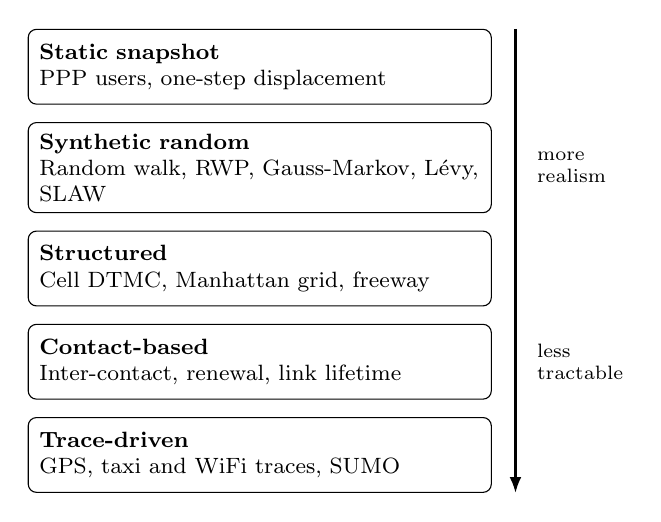
\begin{tikzpicture}[
  fam/.style={draw, rounded corners=3pt, text width=5.6cm, minimum height=0.95cm,
              align=left, font=\footnotesize, inner sep=4pt},
  node distance=0.22cm]
\node[fam] (s) {\textbf{Static snapshot}\\ PPP users, one-step displacement};
\node[fam, below=of s] (r) {\textbf{Synthetic random}\\ Random walk, RWP, Gauss-Markov, L\'evy, SLAW};
\node[fam, below=of r] (m) {\textbf{Structured}\\ Cell DTMC, Manhattan grid, freeway};
\node[fam, below=of m] (c) {\textbf{Contact-based}\\ Inter-contact, renewal, link lifetime};
\node[fam, below=of c] (t) {\textbf{Trace-driven}\\ GPS, taxi and WiFi traces, SUMO};
\draw[-{Latex[length=2mm]}, thick] ([xshift=0.3cm]s.north east) -- ([xshift=0.3cm]t.south east);
\node[font=\scriptsize, align=left, anchor=west] at ([xshift=0.45cm]s.north east |- r.center) {more\\realism};
\node[font=\scriptsize, align=left, anchor=west] at ([xshift=0.45cm]s.north east |- c.center) {less\\tractable};
\end{tikzpicture}

\caption{The five families of mobility models in the edge caching literature. Moving down the list, models keep more of real movement and lose analytical tractability.}
\label{fig:taxonomy}
\end{figure}

\subsection{Static Snapshot Models}
\label{subsec:static}

Stochastic-geometry analyses of caching place base stations, helpers and users as Poisson point processes (PPPs) and evaluate one snapshot of the network. Mobility is absent or enters as a single displacement of each user, as in Krishnan and Dhillon~\cite{krishnan2017mobility}, where each device moves by a distance $v$ between caching and request. The snapshot gives closed forms for hit and coverage probability, but it cannot say how long a user remains in a cell or how often two users meet, which are the quantities proactive and D2D caching depend on.

\subsection{Synthetic Random Models}
\label{subsec:synthetic}

\subsubsection{Random walk}
A user's position evolves as $\mathbf{x}(t)=\mathbf{x}(t-1)+\mathbf{y}_t$ with independent, identically distributed flight vectors $\mathbf{y}_t$. The model is memoryless, and on a torus its stationary spatial distribution is uniform. Our earlier D2D work~\cite{hosny2019performance} used a probabilistic random walk over a set of locations so that meeting probabilities could enter the caching problem in closed form.

\subsubsection{Random waypoint}
Each user picks a destination uniformly in the area, travels to it at a speed drawn from $[v_{\min},v_{\max}]$, pauses, and repeats. Its stationary spatial distribution is not uniform; users concentrate near the center of the area~\cite{bettstetter2004rwp}. Yoon \emph{et al.}~\cite{yoon2003rwp} showed that RWP, as commonly simulated, never reaches a steady state because users spend a growing share of time on slow trips; simulations should start from the stationary distribution or discard a warm-up. Lin \emph{et al.}~\cite{lin2013mobility} defined RWP over the whole plane to remove the boundary effect and derived the handover rate and sojourn time for hexagonal and Poisson base station layouts; the handover rate grows with the square root of base station density. Sojourn time is the window in which a small-cell cache can serve a user, so these results feed directly into a caching model.

\subsubsection{Gauss-Markov}
Speed and direction follow first-order autoregressive processes with a memory parameter $\alpha\in[0,1]$, so that motion changes smoothly instead of turning sharply at waypoints; $\alpha=0$ gives a random walk and $\alpha=1$ straight-line motion~\cite{camp2002survey}. The model needs a rule at the boundary, and that rule changes where users spend their time (Section~\ref{subsec:res-measured}).

\subsubsection{L\'evy walk and SLAW}
Rhee \emph{et al.}~\cite{rhee2011levy} found in GPS traces of people walking outdoors that flight lengths and pause times are heavy-tailed, close to a truncated L\'evy walk. SLAW~\cite{lee2009slaw} keeps these heavy tails and adds regularity: self-similar waypoints, trips planned with the least effort among known places, and a bounded area for each user. No caching analysis in our corpus uses either model, although heavy-tailed pauses decide how often a user is still in the same cell when its request arrives.

\subsection{Structured Models: Markov Chains and Road Maps}
\label{subsec:structured}

Structured models restrict where a user can go next. The common form in proactive caching is a discrete-time Markov chain (DTMC) over cells, helpers or locations with transition matrix $\mathbf{P}$, used for small-cell helpers~\cite{poularakis2013exploiting,poularakis2017code,ozfatura2020mobility} and for D2D users moving among popular locations~\cite{hosny2016allerton}. Vehicular papers replace the abstract chain with a road map: the Manhattan grid~\cite{alnagar2019city}, freeway and city models~\cite{alnagar2022mobility}, and Markov models over RSUs~\cite{wang2024markov}. Yu \emph{et al.}~\cite{yu2021mobility} instead draw vehicle speeds from a truncated Gaussian law with Poisson arrivals at each RSU, which gives the dwell time under the RSU. Structured models are easy to plug into an optimization, but $\mathbf{P}$ is usually assumed known; when it is estimated from data, the estimation error becomes part of the caching problem.

\subsection{Contact-Based Models}
\label{subsec:contact}

For D2D caching, what matters is when two users are close enough to exchange content, so contact-based models describe each pair by the times at which they meet and part. Wang \emph{et al.} use inter-contact times~\cite{wang2017mobility} and an alternating renewal process of contact and inter-contact durations~\cite{wang2018exploiting}. Jarray and Giovanidis~\cite{jarray2016mobility} give each D2D link a random lifetime with mean $\bar{\tau}$, so that a transfer fails if the link breaks before the file arrives. Contact models capture meetings directly but drop positions and base-station association.

\subsection{Trace-Driven and Simulator-Driven Models}
\label{subsec:traces}

Traces replace the model with recorded movement. Public datasets include the GeoLife pedestrian GPS trajectories~\cite{zheng2010geolife} and the San Francisco taxi traces~\cite{piorkowski2009parsimonious}, on which Choi and Lim~\cite{choi2023deep} train an LSTM predictor. Guan \emph{et al.}~\cite{guan2014mobicacher} replay a WiFi access point trace, Mahmood \emph{et al.}~\cite{mahmood2019rich} simulate connected cars in an urban scenario, and the SUMO simulator~\cite{lopez2018sumo} generates vehicle traces for chosen road networks, as in~\cite{wangq2022proactive}. Traces keep daily regularity, the link between place and time, and realistic dwell times. Their cost is that a result holds for one city and period, speed cannot be swept freely, and, when the trace also trains a predictor, the gain mixes the effect of mobility with the accuracy of the predictor.

\begin{table*}[t]
\centering
\caption{Mobility model families in edge caching, ordered from the most abstract to the most realistic}
\label{tab:models}
\footnotesize
\renewcommand{\arraystretch}{1.15}
\setlength{\tabcolsep}{1.8pt}
\def\citepunct{,\,}\def\citedash{--}%  compact citation lists in this table
\begin{tabular*}{\textwidth}{@{\extracolsep{\fill}}llllll@{}}
\hline
Family & Models & Key parameters & Captures & Misses & Caching studies \\
\hline
Static snapshot & PPP with displacement & Density, displacement $v$ & Closed-form coverage & Sojourn, contact times & \cite{krishnan2017mobility} \\
Synthetic random & RW, RWP, GM, L\'evy, SLAW & Speed, pause time, tails & Speed and pause effects & Regularity (except SLAW) & \cite{hosny2019performance} \\
Structured & DTMC, Manhattan, freeway & $\mathbf{P}$, velocity, deadline & Next location; road layout & Error in $\mathbf{P}$; pause tails & \cite{poularakis2013exploiting,poularakis2017code,ozfatura2020mobility,hosny2016allerton,alnagar2019city,alnagar2022mobility,wang2024markov,yu2021mobility} \\
Contact-based & Contacts, link lifetime & Contact rate, $\bar{\tau}$ & Pairwise D2D meetings & Positions; BS association & \cite{wang2017mobility,wang2018exploiting,jarray2016mobility} \\
Trace-driven & GPS, taxi, WiFi; SUMO & Dataset, city, period & Real regularity, dwell times & Free sweeps; generality & \cite{guan2014mobicacher,mahmood2019rich,wangq2022proactive,choi2023deep} \\
\hline
\end{tabular*}
\end{table*}

% ============================================================
% Section 4: How caching problems use mobility
% Counts refer to the 24 caching studies in Table III.
% ============================================================

\section{How Caching Problems Use Mobility}
\label{sec:problems}

Section~\ref{sec:models} asked which mobility model a paper assumes; this section asks what the caching decision does with it. We use three levels:
\begin{itemize}
\item \emph{Mobility-oblivious}: the decision ignores user movement.
\item \emph{Parametric}: the decision uses statistics of the model, such as transition probabilities, contact rates, speed or sojourn time.
\item \emph{Prediction-driven}: the decision uses a forecast of each user's next cell, next RSU or trajectory.
\end{itemize}
Table~\ref{tab:corpus} codes the 24 caching studies of our corpus by architecture, model, level, metric, whether the evaluation varies mobility, and the effect of mobility it reports. Fifteen are parametric, seven prediction-driven, one is oblivious with respect to its users and one does not model mobility. By architecture, eight study vehicular networks, seven D2D, seven small cells and two UAVs. Our search favored papers that mention mobility, so oblivious caching, which is the default in the wider literature~\cite{shanmugam2013femtocaching,maddahali2014fundamental}, is under-represented. % TODO: refresh counts with the final corpus

\begin{table*}[!t]
\centering
\caption{Coded caching studies. Level: P parametric, Pr prediction-driven, O oblivious. Swept: Y the evaluation varies a mobility parameter, N it does not, ? not yet checked. n.c.: not coded}
\label{tab:corpus}
\scriptsize
\renewcommand{\arraystretch}{1.1}
\begin{tabular}{lllllll}
\hline
Ref. & Architecture & Mobility model & Level & Gain metric & Swept & Reported effect \\
\hline
\cite{poularakis2013exploiting} & Small cells, coded & DTMC over helpers, deadline & P & Macro-cell requests & ? & n.c. \\
\cite{poularakis2017code} & Dense small cells & Markov random walk, human traces & Pr & Macro-cell load & ? & n.c. \\
\cite{ozfatura2020mobility} & Small cells, coded & DTMC on a grid & P & Backhaul load & Y & Raises load if less predictable \\
\cite{semiari2018caching} & mmW/$\mu$W HetNet & User speed through small cells & P & Handover failures, energy & ? & Mitigated by caching \\
\cite{guan2014mobicacher} & Small cells & Known or predicted trajectories, WiFi trace & Pr & Caching utility & ? & n.c. \\
\cite{tadrous2016optimal} & Cellular & Not modeled (demand uncertainty) & -- & Service cost & -- & -- \\
\cite{abani2017proactive} & ICN edge & Prediction with uncertainty & Pr & n.c. & ? & n.c. \\
\hline
\cite{krishnan2017mobility} & D2D & PPP with displacement & P & Coverage, local delay & Y & Helps \\
\cite{jarray2016mobility} & D2D & Random link lifetime & P & Service success probability & Y & Hurts \\
\cite{wang2017mobility} & D2D & Inter-contact times & P & Offloading ratio & Y & Non-monotone in speed \\
\cite{wang2018exploiting} & D2D & Alternating renewal & P & Offloading ratio & Y & Helps \\
\cite{hosny2016allerton} & D2D & Periodic DTMC over locations & P & Service cost & N & Helps \\
\cite{hosny2016globecom} & D2D & n.c. & P & n.c. & ? & n.c. \\
\cite{hosny2019performance} & D2D & Probabilistic random walk & P & Service cost & ? & n.c. \\
\hline
\cite{alnagar2019city} & RSU & Manhattan city model & P & Latency & ? & n.c. \\
\cite{alnagar2022mobility} & RSU & Freeway and city models & P & Latency & ? & n.c. \\
\cite{tan2018mobility} & Vehicular & Mobility-aware reward & P & Operational cost & ? & n.c. \\
\cite{mahmood2019rich} & Edge nodes, cars & Dwell time and paths, urban traces & P & Throughput, hit probability & Y & n.c. \\
\cite{wang2024markov} & RSU & Markov mobility model & P & Hit rate & Y & n.c. \\
\cite{yu2021mobility} & RSU & Truncated Gaussian speed, Poisson arrivals & Pr & Hit ratio & N & Hurts (stated) \\
\cite{wangq2022proactive} & RSU & SUMO traces of two cities & Pr & Next-RSU accuracy & N & n.c. \\
\cite{choi2023deep} & RSU, vehicles & San Francisco taxi traces, LSTM & Pr & Throughput, delay, cost & N & Hurts (stated) \\
\hline
\cite{chen2017sky} & UAV & ESN prediction, BUPT pedestrian traces & Pr & QoE, transmit power & N & n.c. \\
\cite{xu2018overcoming} & UAV, static nodes & UAV trajectory, nodes static & O & Caching and delivery time & -- & -- \\
\hline
\end{tabular}
\end{table*}

\subsection{Parametric Caching}
\label{subsec:parametric}

Parametric schemes are the majority and include almost all analytical work. Their models were described in Section~\ref{sec:models}; at the decision level they differ in what they optimize. Small-cell schemes place coded segments so that a user collects a file from the helpers it visits before a deadline~\cite{poularakis2013exploiting,ozfatura2020mobility}. Semiari \emph{et al.}~\cite{semiari2018caching} reverse the direction: a fast user caches content ahead of time so that it can skip a handover into a millimeter wave small cell. D2D schemes choose what each device stores given contact or meeting statistics~\cite{wang2017mobility,wang2018exploiting,hosny2016allerton,hosny2019performance}. Vehicular schemes fold speed, dwell time or the sequence of RSUs into the placement~\cite{alnagar2019city,alnagar2022mobility,mahmood2019rich,wang2024markov} or into the reward of a reinforcement learning agent~\cite{tan2018mobility}. Their common weakness is that the parameters are taken as known; few test how the placement degrades when they are wrong.

\subsection{Prediction-Driven Caching}
\label{subsec:prediction}

Prediction-driven schemes forecast where each user goes next and cache accordingly, using mobility predictions with network coding~\cite{poularakis2017code}, known or predicted trajectories~\cite{guan2014mobicacher}, echo state networks for UAV placement~\cite{chen2017sky}, federated learning~\cite{yu2021mobility}, bandit learning of the next RSU~\cite{wangq2022proactive}, or LSTM trajectory prediction~\cite{choi2023deep}. Prediction error is the central risk. Abani \emph{et al.}~\cite{abani2017proactive} hedge by caching beyond the edge, and Mahmood \emph{et al.}~\cite{mahmood2019rich} find that only large errors in dwell time and path visibly affect performance. Tadrous and Eryilmaz~\cite{tadrous2016optimal} bound the cost of proactive caching under demand-prediction uncertainty; the corresponding bound for mobility-prediction uncertainty is not available in the coded papers.

\subsection{Mobility-Oblivious Caching}
\label{subsec:oblivious}

An oblivious scheme evaluated under mobility shows how much a mobility-aware design adds, and Section~\ref{sec:benchmark} uses most-popular caching for this purpose. Xu \emph{et al.}~\cite{xu2018overcoming} illustrate a second kind of mobility: the ground nodes are static, and the UAV pushes content into their caches while in range so that requests can be served after it leaves.

% ============================================================
% Section 5: Effect of mobility on the caching gain
% ============================================================

\section{Effect of Mobility on the Caching Gain}
\label{sec:effect}

The coded studies disagree on whether mobility raises or lowers the caching gain. Some find that it helps~\cite{krishnan2017mobility,wang2018exploiting,guan2014mobicacher,alnagar2022mobility}, some that it hurts~\cite{jarray2016mobility,semiari2018caching}, and one that the best placement shifts with speed in a non-monotone way~\cite{wang2017mobility}. We trace the disagreement to four mechanisms, summarized in Table~\ref{tab:mechanisms}, and each model contains only some of them.

\begin{table*}[t]
\centering
\caption{Mechanisms through which mobility changes the caching gain}
\label{tab:mechanisms}
\footnotesize
\renewcommand{\arraystretch}{1.2}
\begin{tabular}{llll}
\hline
Mechanism & Sign & When it dominates & Evidence \\
\hline
New contacts and new caches & Raises gain & Short transfers; sparse caches with different contents & \cite{krishnan2017mobility,wang2018exploiting,hosny2016allerton,poularakis2013exploiting} \\
Interrupted delivery & Lowers gain & Transfers long relative to contact or sojourn time; high speed & \cite{jarray2016mobility,semiari2018caching,yu2021mobility,mahmood2019rich} \\
Duplication versus diversity & Either & Number of distinct caches met before the deadline & \cite{wang2017mobility,ozfatura2020mobility} \\
Unpredictable movement & Lowers mobility-aware gain & High transition entropy, prediction error, model mismatch & \cite{ozfatura2020mobility,abani2017proactive,mahmood2019rich} \\
\hline
\end{tabular}
\end{table*}

\subsection{New Contacts and New Caches}
\label{subsec:mech-contacts}

A moving user meets more peers and passes more cells within a deadline than a static one, and each new contact is another chance to find the file. Under an alternating renewal model, the D2D offloading ratio provably increases with speed~\cite{wang2018exploiting}. Displacing users between caching and request improves coverage and local delay~\cite{krishnan2017mobility}, and higher meeting probabilities raise the proactive gain in our D2D model~\cite{hosny2016allerton}. In small cells, collecting coded segments from all helpers visited before the deadline is what makes mobility useful~\cite{poularakis2013exploiting}. The mechanism assumes that contacts last long enough and that the caches met hold different content; the next two mechanisms remove these assumptions.

\subsection{Interrupted Delivery}
\label{subsec:mech-interrupt}

When a contact or a sojourn ends before the file arrives, the transfer is lost. With random link lifetimes, higher mobility lowers the service success probability, and small files fare better than large ones~\cite{jarray2016mobility}. At the cell level, fast users crossing millimeter wave small cells suffer handover failures, which caching can partly avoid~\cite{semiari2018caching}. Vehicular papers name the short dwell time under an RSU as the main obstacle~\cite{yu2021mobility}, and RICH stores content where cars move slowly, such as congested intersections, because that is where they have time to download~\cite{mahmood2019rich}. Which of the first two mechanisms wins is set by the ratio of transfer time to contact or sojourn time; Section~\ref{subsec:res-d2d} measures the crossover.

\subsection{Duplication Versus Diversity}
\label{subsec:mech-diversity}

If every cache stores the same popular files, meeting more caches adds nothing. Wang \emph{et al.}~\cite{wang2017mobility} show that users moving very slowly or very fast should cache the most popular files, while users at medium speed should cache less popular ones to avoid duplication. Our reading is that diversity pays only when a user meets several distinct caches before the deadline, but not so many that the popular files are within reach anyway. Ozfatura and G\"und\"uz~\cite{ozfatura2020mobility} find similarly that the value of spreading coded segments depends on how many cells a user can reach. The reported effect of mobility therefore depends on the caching policy as well as the model: most-popular caching sees little benefit from mobility, a diversity-seeking placement can see a large one.

\subsection{Unpredictable Movement}
\label{subsec:mech-predict}

Under a DTMC, the backhaul load rises as mobility becomes less predictable~\cite{ozfatura2020mobility}, so two networks with the same mean speed can give different gains. Prediction error (Section~\ref{subsec:prediction}) and model mismatch, a placement tuned to one model and used under another, act through this mechanism; Section~\ref{subsec:mismatch} measures the cost of mismatch.

\subsection{How Strong Is the Evidence?}
\label{subsec:evidence}

Of the 24 coded studies, 9 vary a mobility parameter in their evaluation, 10 do not, 3 could be coded only from the abstract, and 2 do not apply (Table~\ref{tab:corpus}). Two of the studies that do not vary mobility still describe it as harmful from the model alone~\cite{yu2021mobility,choi2023deep}. The well-supported results come from a few D2D and small-cell analyses. In vehicular and UAV caching, where speeds are highest, only two studies vary mobility~\cite{alnagar2022mobility,wang2024markov}, and only one of them reports how the gain responds. The studies that do vary mobility also differ in model, metric, delivery requirement and policy, each of which can change the sign of the effect. Section~\ref{sec:benchmark} fixes all but the model.

% ============================================================
% Section 6: Unified benchmark
% All numbers come from benchmark/results/raw.csv (10 seeds per point),
% d2d_prediction.csv, mismatch_v5.mat and rwp_warmup_v5.mat
% (MATLAB code in benchmark/).
% ============================================================

\section{A Unified Benchmark of Mobility Models}
\label{sec:benchmark}

To separate the factors identified in Section~\ref{sec:effect}, we built one benchmark in which the network, content, requests and caching policies are fixed and only the mobility model changes. Beyond comparing models, we ask which measured property of the mobility determines the gain, so that a result obtained under one model can be carried over to another. The MATLAB code runs unchanged in GNU Octave and is released with the paper.

\subsection{Setup}
\label{subsec:setup}

Table~\ref{tab:params} lists the parameters. Two hundred users move in a 1~km $\times$ 1~km area served by a $5\times5$ grid of small base stations (SBSs), each covering a 200~m $\times$ 200~m cell; a user is associated with the SBS of the cell it is in. Each user sends requests as a Poisson process with rate $1/120$ per second, for files drawn from the Zipf law~\eqref{eq:zipf} with $N=1000$ and $\gamma=0.8$. Each SBS stores $C=50$ files. Each user stores $c=10$ distinct files, drawn with probability proportional to popularity, and can serve peers within 50~m.

A request must be delivered within $T_d=60$~s. Following~\eqref{eq:effhit}, delivery from an SBS needs $D_s=10$~s of uninterrupted association with an SBS that holds the file, and delivery over D2D needs $D_d$ seconds of uninterrupted contact with a peer that holds it, with $D_d$ between 2 and 30~s. A request for a file in the user's own cache counts as offloaded.

\begin{table*}[t]
\centering
\caption{Benchmark parameters}
\label{tab:params}
\footnotesize
\renewcommand{\arraystretch}{1.1}
\begin{tabular}{ll@{\hspace{0.6cm}}ll}
\hline
Parameter & Value & Model & Setting \\
\hline
Area, users & 1~km $\times$ 1~km, $U=200$ & Random walk & New direction every 30~s; reflection at the walls \\
SBSs & $5\times5$ grid, 200~m cells & RWP & Speed $\sim U[0.5v,1.5v]$, pause $\sim U[0,60]$~s \\
Library, popularity & $N=1000$, Zipf $\gamma=0.8$ & Gauss-Markov & $\alpha=0.85$, $\sigma_v=0.3v$, $\sigma_\theta=\pi/4$; steering and reflection at the walls \\
SBS cache, user cache & $C=50$, $c=10$ files & Markov cell & Stay w.p.\ 0.3, else a random neighbor; random point in cell \\
Request rate & $1/120$ per user per second & Manhattan & 100~m blocks; straight 0.5, left 0.25, right 0.25 \\
Deadline $T_d$ & 60~s & L\'evy walk & Tails $\alpha=\beta=1.5$; flights 10--1000~m, pauses 10--1800~s \\
SBS delivery time $D_s$ & 10~s & & \\
D2D range, transfer time $D_d$ & 50~m; 2, 5, 10, 20, 30~s & & \\
Travel speed $v$ & 0.5, 1, 2, 5, 10, 20~m/s & & \\
Measured period, warm-up & 3600~s, 2000~s discarded & & \\
Seeds & 10 per configuration & & \\
\hline
\end{tabular}
\end{table*}

\emph{Mobility models.} We implement seven models from the synthetic and structured families of Section~\ref{sec:models}: static users, random walk, RWP, Gauss-Markov, a Markov chain over cells, a Manhattan grid and a truncated L\'evy walk. The parameter $v$ is the speed while moving. Users that reach a wall are reflected, and movement is interpolated at 1~s resolution so that a reflected path does not cut corners. The L\'evy parameters are illustrative and are not fitted to the traces of~\cite{rhee2011levy}. Trace-driven runs are not included; the code accepts a trace in place of a generator.

\emph{Caching policies.} Three SBS policies are compared.
\begin{itemize}
\item \emph{Most popular (MPC)}: every SBS stores the $C$ most popular files. It ignores mobility.
\item \emph{Mobility-aware (MA)}: a greedy placement that uses the \emph{reach matrix} $\mathbf{W}$, where $W_{bb'}$ is the probability that a user at SBS $b$ at a request instant stays with SBS $b'$ for $D_s$ seconds before the deadline. With $\pi_b$ the share of time spent at $b$ and $x_{b'f}\in\{0,1\}$ the placement, the greedy step maximizes
\begin{equation}
\sum_{b}\pi_b\sum_{f}p_f\Big[1-\prod_{b'}\big(1-x_{b'f}W_{bb'}\big)\Big],
\label{eq:maobj}
\end{equation}
treating visits as independent, until every cache is full. $\mathbf{W}$ and $\pi$ are estimated from an independent run of the same model, as an operator would learn them from history. The scheme is an uncoded relative of the helper placement in~\cite{poularakis2013exploiting}.
\item \emph{LRU}: each SBS runs least-recently-used replacement on the requests it receives and serves only users currently associated with it.
\end{itemize}
D2D caches keep the fixed popularity-proportional placement, so that changes in D2D offloading come from mobility alone. We report the snapshot and effective hit ratios of Section~\ref{subsec:metrics} and the D2D offloading ratio.

\emph{Statistics.} Each configuration runs for one measured hour with 10 independent seeds. Figures show the mean with 95\% confidence intervals; the half-width is at most 0.006 for every hit and offloading ratio. Every run discards a 2000~s warm-up. The warm-up matters for RWP: started with speeds in $(0,2v]$ and uniform positions~\cite{yoon2003rwp}, our RWP at $v=5$~m/s slowed from 2.4~m/s in its first 20 minutes to 1.3~m/s in its fourth hour, and its D2D offloading ratio drifted from 0.29 to 0.25 for $D_d=2$~s and from 0.13 to 0.15 for $D_d=30$~s (three seeds). The benchmark RWP uses a positive minimum speed and the warm-up, and stays at 3.6~m/s.

\subsection{Measured Mobility}
\label{subsec:res-measured}

\begin{table}[t]
\centering
\caption{Measured mobility statistics at $v=5$~m/s}
\label{tab:stats}
\footnotesize
\renewcommand{\arraystretch}{1.1}
\setlength{\tabcolsep}{2.2pt}
\begin{tabular}{lrrrrrr}
\hline
Model & Speed & Sojourn & Handover & Contact & Inter- & Reach \\
 & (m/s) & (s) & (per h) & (s) & contact (s) & \\
\hline
Random walk & 4.99 & 39.2 & 91.0 & 12.6 & 517 & 1.77 \\
RWP & 3.60 & 45.2 & 79.1 & 14.5 & 826 & 1.81 \\
Gauss-Markov & 5.00 & 36.2 & 98.6 & 11.9 & 435 & 1.73 \\
Markov cell & 4.97 & 52.4 & 68.4 & 12.7 & 589 & 1.74 \\
Manhattan & 5.00 & 49.8 & 71.8 & 19.9 & 785 & 1.79 \\
L\'evy walk & 0.81 & 193.6 & 15.0 & 50.8 & 245 & 1.15 \\
\hline
\end{tabular}
\end{table}

Table~\ref{tab:stats} reports, at $v=5$~m/s, the measured mean speed including pauses, the mean sojourn time in a cell, the handover rate, the mean contact and inter-contact durations of a user pair, and the \emph{reach}: the mean number of distinct SBSs with which a user, at a random instant, stays for at least $D_s$ within the next $T_d$. At the same nominal speed the models differ widely. The mean inter-contact time ranges from 435~s (Gauss-Markov) to 826~s (RWP), and the L\'evy walk, whose heavy-tailed pauses dominate, moves at 0.81~m/s on average. The spatial distribution also differs. RWP users concentrate near the center~\cite{bettstetter2004rwp}: at 2~m/s, 18.6\% of user-time falls in the central 300~m $\times$ 300~m square, which is 9\% of the area. With the steering rule of Table~\ref{tab:params}, Gauss-Markov users avoid the border at low speed and occupy it uniformly at 20~m/s. The rest of this section shows which of these statistics the gain depends on.

\subsection{Small-Cell Caching}
\label{subsec:res-sbs}

\begin{figure*}[t]
\centering
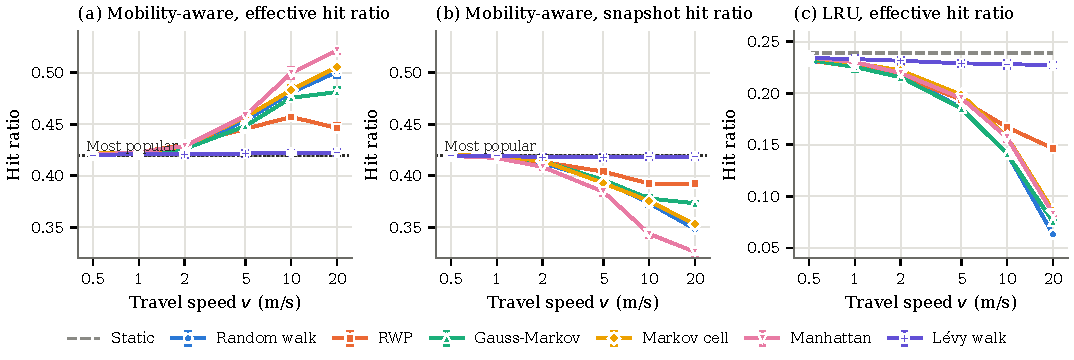
\includegraphics[width=\textwidth]{figures/fig_sbs_hit.pdf}
\caption{SBS caching. (a)--(c) Hit ratios against travel speed, mean of 10 seeds with 95\% confidence intervals; the dotted line is MPC (0.420). (d) Gain of the mobility-aware placement over MPC against the measured reach, one point per model and speed; the dotted reference line is fitted through the origin to all moving models except RWP.}
\label{fig:sbs}
\end{figure*}

\emph{Replication makes the gain immune to handovers.} Under MPC every SBS holds the same files, so any 10~s stay with any SBS completes the delivery. Its effective hit ratio is 0.418 to 0.420 under all models and speeds.

\emph{Diversity turns mobility into gain.} At 0.5~m/s the mobility-aware placement performs like MPC under every model (0.420 to 0.422). At 20~m/s its effective hit ratio is 0.522 under the Manhattan model, 0.505 under the Markov cell model, 0.501 under the random walk and 0.481 under Gauss-Markov, gains of 24.3\%, 20.4\%, 19.4\% and 15.1\% over MPC (Fig.~\ref{fig:sbs}a). Under RWP the gain peaks at 8.9\% at 10~m/s and falls to 6.4\% at 20~m/s; under the L\'evy walk it never exceeds 0.7\%.

\emph{Reach explains most of the spread.} Fig.~\ref{fig:sbs}d plots the gain of every model and speed against the reach. The correlation is 0.98, and for all moving models except RWP the gain grows by about 10.4\% for each additional SBS within reach. Nominal speed does not order the points; the L\'evy walk at 20~m/s has the reach (1.16) and the gain (0.7\%) of the other models at 1~m/s. RWP falls below the line. At 5~m/s it has the highest reach of all models (1.81) but a lower gain (6.2\%) than every model except the L\'evy walk. Its users concentrate in the center, so the cells they reach are mostly the same central cells: 56\% of the off-diagonal reach of $\mathbf{W}$ points to the central nine cells, against 38\% to 46\% for the other moving models (mean of 10 seeds). A central cache serves users from several neighbors and cannot complement each of them, so the reach of RWP buys less diversity. The gain therefore depends on how many caches a user reaches and on how evenly those caches are shared.

\emph{The snapshot metric reverses the conclusion.} The snapshot hit ratio of the same placement falls below MPC as speed grows, to 0.326 under the Manhattan model at 20~m/s, 22.3\% below MPC (Fig.~\ref{fig:sbs}b). A paper that reported only the snapshot ratio would conclude that the mobility-aware placement is worse than MPC, while the effective ratio shows it is 24.3\% better. The snapshot ratio counts only the cache at the request instant, so it penalizes a placement that relies on the next cells for the files it does not hold.

\emph{Reactive caching at the serving cell loses deliveries to handovers.} LRU serves a user only from the cell it is in at the request instant. Its effective hit ratio drops from 0.239 for static users to between 0.063 (random walk) and 0.146 (RWP) at 20~m/s, and stays at 0.227 under the L\'evy walk (Fig.~\ref{fig:sbs}c). Its snapshot ratio stays between 0.235 and 0.240 throughout, and the product of the snapshot ratio and the probability that a user stays at least $D_s$ in its current cell reproduces the effective ratio within 0.003 for every model and speed. The loss is thus the interruption mechanism of Section~\ref{subsec:mech-interrupt}, and it is set by one sojourn statistic.

\subsection{D2D Caching}
\label{subsec:res-d2d}

\begin{figure*}[t]
\centering
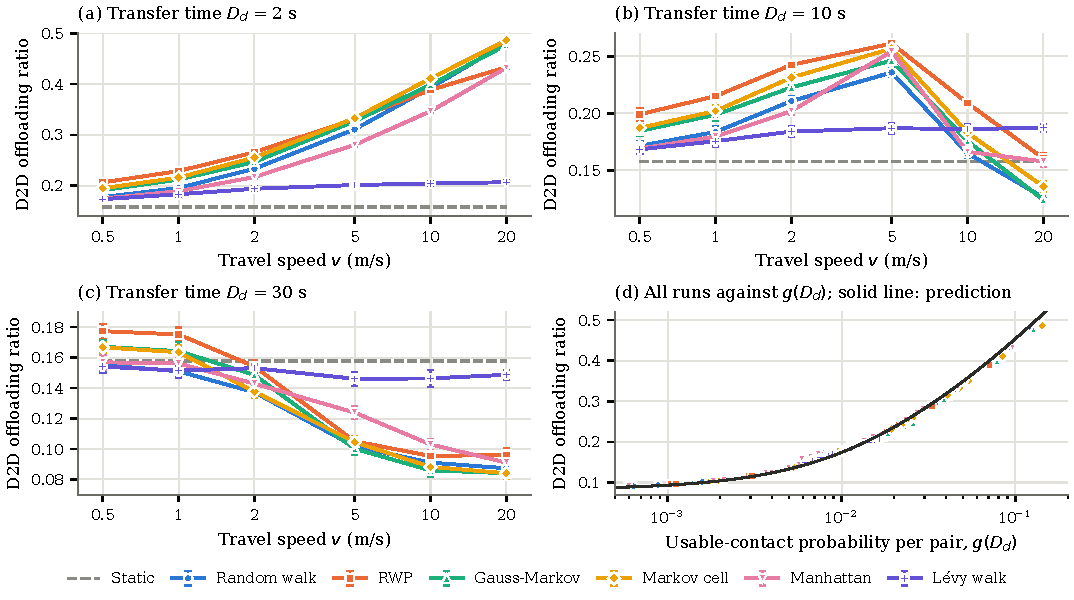
\includegraphics[width=\textwidth]{figures/fig_d2d.pdf}
\caption{D2D offloading. (a)--(c) Offloading ratio against travel speed for short, medium and long transfers, mean of 10 seeds with 95\% confidence intervals; the dashed line is the static network (0.158). (d) Offloading ratio of all 210 configurations (seven models, six speeds, five transfer times) against the usable-contact probability $g(D_d)$ of~\eqref{eq:gdd}; the solid line is the prediction~\eqref{eq:d2dpred}.}
\label{fig:d2d}
\end{figure*}

Fig.~\ref{fig:d2d}a--c reproduces the three conclusions found in the literature, in one setting, by changing only the transfer time.

\emph{Short transfers: mobility helps.} With $D_d=2$~s, offloading grows with speed under every moving model, from 0.158 for static users to between 0.432 (Manhattan) and 0.486 (Markov cell) at 20~m/s; the L\'evy walk reaches only 0.207. This agrees with the renewal-model result that offloading increases with speed~\cite{wang2018exploiting}.

\emph{Long transfers: mobility hurts.} With $D_d=30$~s, offloading falls with speed and, for every model except the L\'evy walk, drops to between 0.084 and 0.096 at 20~m/s, below the static network. At that speed contacts last 3 to 5~s on average. This agrees with the link-lifetime result that higher mobility lowers the success probability~\cite{jarray2016mobility}.

\emph{Medium transfers: the effect is non-monotone.} With $D_d=10$~s, offloading under every model except the L\'evy walk rises to between 0.236 and 0.261 at 5~m/s, where the mean contact lasts 12 to 20~s, and falls to between 0.124 and 0.161 at 20~m/s. Wang \emph{et al.} found a non-monotone dependence on speed in the optimal placement~\cite{wang2017mobility}; here it appears in the offloading ratio of a fixed placement.

\emph{One contact statistic predicts the offloading ratio.} These three regimes follow from a single quantity. Let $h_l$ be the number of contacts of length $l$ seconds per user pair over a period of $T$ seconds. If contacts form a stationary sequence, the probability that a pair offers at least $D_d$ consecutive seconds of contact within a window of $T_d$ seconds that starts at a random instant is approximately
\begin{equation}
g(D_d)=\frac{1}{T}\sum_{l\ge D_d} h_l\,\big[(l-D_d+1)+(T_d-D_d)\big].
\label{eq:gdd}
\end{equation}
The first term counts windows that open during a contact with at least $D_d$ seconds left; the second counts contacts long enough that start early enough in the window. Let $q_f$ be the probability that a user caches file $f$. If the $U-1$ other users act independently, the offloading ratio is
\begin{equation}
\rho=\sum_f p_f\Big[q_f+(1-q_f)\big(1-(1-g\,q_f)^{U-1}\big)\Big].
\label{eq:d2dpred}
\end{equation}
For static users $g$ is the fraction of pairs in range. We computed $g$ from the contact histogram of each run and compared~\eqref{eq:d2dpred} with the simulated ratio. Over the 210 configurations the mean absolute error is 0.004, 90\% of the errors are below 0.01, and the largest is 0.027, for the Markov cell model at 20~m/s with $D_d=2$~s, where many concurrent contacts make the independence assumption optimistic. All configurations fall on one curve (Fig.~\ref{fig:d2d}d): once $g(D_d)$ is known, neither the model nor the speed adds information.

Equation~\eqref{eq:gdd} also explains the crossover. For a short transfer, $g$ is close to the contact rate times $T_d$ and grows with speed. For a long one, only contacts longer than $D_d$ count, and their number falls as speed shortens contacts. The L\'evy walk is flat because its long pauses keep contacts long at every speed, and RWP gives the highest offloading among the moving models at low speed because its central concentration raises the contact rate. A mobility model therefore enters D2D caching only through its contact-length distribution, which can be measured from a trace and reported in a paper.

\subsection{Training on the Wrong Model}
\label{subsec:mismatch}

\begin{table}[t]
\centering
\caption{Effective hit ratio when the mobility-aware placement is trained on one model (rows) and used under another (columns), $v=5$~m/s, mean of 10 seeds. MPC gives 0.420 in every column.}
\label{tab:mismatch}
\footnotesize
\renewcommand{\arraystretch}{1.1}
\setlength{\tabcolsep}{2.6pt}
\begin{tabular}{lccccccc}
\hline
Train $\backslash$ Test & Stat. & RW & RWP & GM & MC & MH & L\'evy \\
\hline
Static & \textbf{.420} & .420 & .420 & .420 & .420 & .420 & .420 \\
Random walk & .394 & \textbf{.454} & .451 & .449 & .453 & .457 & .404 \\
RWP & .398 & .446 & \textbf{.445} & .444 & .449 & .451 & .409 \\
Gauss-Markov & .399 & .450 & .450 & \textbf{.448} & .454 & .454 & .409 \\
Markov cell & .391 & .451 & .449 & .449 & \textbf{.457} & .457 & .404 \\
Manhattan & .385 & .451 & .449 & .449 & .452 & \textbf{.458} & .397 \\
L\'evy walk & .418 & .434 & .434 & .434 & .436 & .436 & \textbf{.421} \\
\hline
\end{tabular}
\end{table}

Table~\ref{tab:mismatch} trains the mobility-aware placement on one model and uses it under another, at 5~m/s. Training on static users reproduces MPC, as it should, since $\mathbf{W}$ is then the identity. The 95\% confidence half-width of every entry is below 0.006.

Among the five models in which users keep moving, mismatch costs little: in every column, the worst cross-model entry is within 0.009 of the matched one. In the RWP column every cross-trained placement does better than the one trained on RWP (0.449 to 0.451 against 0.445). This is the effect seen in Fig.~\ref{fig:sbs}d from the other side: RWP reach is concentrated on shared central cells, which~\eqref{eq:maobj} treats as independent visits, so a placement learned from more uniform movement spreads content better.

Mismatch is costly when the training model moves and the actual users mostly do not. A placement trained on any of the five moving models and used with static users gives 0.385 to 0.399, 5.0\% to 8.2\% below MPC; used with L\'evy walkers it gives 0.397 to 0.409, again below MPC. Training on the L\'evy walk is safe but timid: it is never more than 0.002 below MPC, and on moving users it gives 0.434 to 0.436 against 0.445 to 0.458 for the matched placements. What matters is therefore the regime, moving or pause-dominated, more than the model. A mobility-aware placement should be trained on mobility of the same regime as its users, and when the population mixes both, it should be checked against the oblivious baseline, because a diversity-seeking placement can do worse than MPC for users who stay put.

% ============================================================
% Section 7: Lessons learned and reporting recommendations
% ============================================================

\section{Lessons Learned and Reporting Recommendations}
\label{sec:lessons}

Read together, the survey and the benchmark show that a reported effect of mobility depends on four choices besides the mobility itself: the model, the caching policy, the delivery requirement and the metric. The benchmark also shows that the model name and the nominal speed are the wrong description of mobility. What the gain depends on is a small set of measured statistics: the reach of a user over the deadline for small-cell placement, the probability of staying in the current cell for reactive caching, and the contact-length distribution for D2D caching. Models that agree on these statistics give the same gain, and models that disagree on them give different gains at the same speed. This leads to four recommendations.

\emph{Report the mobility a cache sees, not only the model.} A paper should give every model parameter, including pause times, boundary handling and how the initial state is set, and should report the measured statistics that drive the gain: mean speed including pauses, sojourn time per cell, reach over the deadline, and the contact and inter-contact durations. For traces, the dataset, area, period and preprocessing are also needed. With these statistics, a result can be compared with one obtained under a different model or trace.

\emph{Use a delivery-aware metric.} The snapshot hit ratio can rank two placements in the opposite order to the effective hit ratio (Section~\ref{subsec:res-sbs}). The delivery time and the deadline should be stated with the metric.

\emph{Compare against oblivious baselines under the same mobility.} A replicating policy such as MPC is immune to handovers, and a reactive policy such as LRU loses deliveries to them. Reporting both shows how much of the gain comes from using mobility and how much from the baseline's exposure to it.

\emph{Vary mobility and test robustness.} A mobility parameter should be swept over the range of the target users, since the sign of the effect can change within that range (Section~\ref{subsec:res-d2d}). A mobility-aware or prediction-driven scheme should also be tested under mobility other than the one it was trained on (Section~\ref{subsec:mismatch}).

\emph{Limits.} The corpus of 24 coded studies is a draft sample, and several rows are coded from abstracts. The benchmark uses one network size, popularity that is the same in every cell, uncoded caching and synthetic mobility only; each can be changed in the released code, and trace-driven runs are the most important addition. The predictor~\eqref{eq:d2dpred} assumes independent holders and a stationary contact sequence. Absolute hit ratios depend on the chosen cache sizes and popularity skew, so the conclusions concern how the gain responds to mobility. % TODO: remove the corpus caveat once the corpus is final

% ============================================================
% Section 8: Open problems
% ============================================================

\section{Open Problems}
\label{sec:open}

\subsection{Traces That Can Be Shared and Swept}
Trace-driven evaluation keeps the regularity of real movement, but a result holds for one city and one period, and the trace cannot be slowed down or sped up. The public datasets that appear in the caching literature are few: pedestrian GPS trajectories~\cite{zheng2010geolife}, taxi traces~\cite{piorkowski2009parsimonious}, and simulator output from SUMO~\cite{lopez2018sumo}. Several papers rely on traces that are not public. Section~\ref{sec:benchmark} suggests a practical middle path. The gain depends on a few statistics: the reach over the deadline, the probability of staying in the current cell, and the contact-length distribution. A synthetic model fitted to these statistics of a trace should reproduce the gain of the trace and can still be swept. Testing this on public traces is the next step.

\subsection{Mobility-Prediction Uncertainty}
Proactive caching under demand uncertainty has fundamental bounds~\cite{tadrous2016optimal}. The corresponding bounds for uncertainty in where users will be are missing, even though prediction-driven schemes are common in vehicular and UAV caching. Robustness is usually tested, if at all, by perturbing one input~\cite{mahmood2019rich}. Section~\ref{subsec:mismatch} shows that training on the wrong mobility model can erase the advantage of a mobility-aware placement, so a bound that couples the prediction error with the caching gain would be directly useful in practice.

\subsection{Joint Mobility and Demand}
Most papers, and our benchmark, draw requests from one popularity law everywhere. When demand depends on place and time, as it does for location-based content, mobility changes both where a request is served and what is requested. Models that couple the two are rare.

\subsection{Human-Like and Mixed Mobility}
L\'evy walks and SLAW reproduce the heavy-tailed flights and pauses observed in GPS traces~\cite{rhee2011levy,lee2009slaw}, yet no coded caching analysis uses them. Real cells also mix pedestrians, cars and buses, and people often move in groups, as in the group mobility models reviewed by Camp \emph{et al.}~\cite{camp2002survey}. How these mixtures change contact and sojourn statistics, and hence the gain, is unexplored.

\subsection{Two Moving Tiers}
UAV caching adds a second source of mobility. Some papers move the cache to follow predicted user positions~\cite{chen2017sky}; others plan the UAV path over static users~\cite{xu2018overcoming}. A cache that moves while its users also move, with both trajectories partly controllable or predictable, has not been analyzed in the coded literature.

\subsection{Delivery-Aware Metrics and Coded Delivery}
The snapshot hit ratio hides the effect of mobility on delivery (Section~\ref{subsec:metrics}). Coded and segmented delivery can turn an interrupted transfer into a partial one that another cache completes~\cite{poularakis2013exploiting,ozfatura2020mobility}. Coded delivery has so far been evaluated under one mobility model per paper, so how much of an interrupted transfer it recovers under different contact and sojourn statistics is not known.

\subsection{Caching Beyond Files}
Edge caches increasingly hold computation results, machine learning models and compact semantic representations of content instead of complete files. These items are small, and their value depends on the user's context, which in turn depends on where the user is. A cached item may therefore lose its value when the user moves, even if the user stays within reach of the cache. How mobility interacts with such caches, including caches that run on low-power embedded hardware at the edge, is not addressed by the file-centric literature surveyed here.

% ============================================================
% Section 9: Conclusion
% ============================================================

\section{Conclusion}
\label{sec:conclusion}

We surveyed how edge caching models user mobility, classified 24 caching studies by model and by how their decisions use mobility, and explained their conflicting findings through four mechanisms. The question in the title has no single answer. Mobility can help or hurt, and a MATLAB benchmark with seven mobility models shows when.

\emph{Small-cell caching.} Mobility helps a placement that spreads different files over neighboring cells. Its gain over most-popular caching ranges from 0.7\% to 24.3\% across models at the same nominal speed and grows by about 10.4\% for each additional cell a user can reach before the deadline. Mobility hurts reactive caching at the serving cell, which loses exactly the deliveries that a handover interrupts.

\emph{D2D caching.} Mobility helps short transfers and hurts long ones, and in between the effect is non-monotone. The offloading ratio follows from the contact-length distribution through a closed-form expression, with a mean error of 0.004.

\emph{Evaluation choices.} The metric and the user population can reverse a conclusion. The snapshot hit ratio reports a loss where deliveries show a gain, and when most users are static the mobility-aware gain nearly disappears while a placement trained on moving users does worse than most-popular caching.

Results obtained under different models become comparable once a paper reports the reach, the probability of staying in the current cell and the contact-length distribution, together with a delivery-aware hit ratio (Section~\ref{sec:lessons}). The most pressing open problems are trace-calibrated models that can still be swept and bounds on the gain under mobility-prediction error (Section~\ref{sec:open}).


\section*{Code and Data Availability}
The MATLAB benchmark (which runs in MATLAB and GNU Octave), all raw results, the coding sheet of the surveyed studies and the source of this paper are available at \url{https://github.com/sshawky78AUA/mobility-edge-caching}. The code is released under the MIT license and the data under CC BY 4.0.

\bibliographystyle{IEEEtran}
\bibliography{refs}

\end{document}
